\documentclass[11pt,a4paper]{article}

% ============================================================
% PAQUETES BÁSICOS
% ============================================================
\usepackage[backend=biber,style=apa]{biblatex}
\usepackage{csquotes}
\usepackage{fontspec}
\setmainfont{Myriad Pro}    % Fuente principal
\usepackage[spanish]{babel}
\usepackage{graphicx}
\usepackage{geometry}
\usepackage{fancyhdr}
\usepackage{titlesec}
\usepackage{xcolor}
\usepackage{hyperref}
\usepackage{amsmath}        % Para ecuaciones matemáticas
\usepackage{float}          % Para mejor control de posición de figuras
\usepackage{caption}        % Para personalizar captions
\usepackage{subcaption}     % Para subfiguras si se necesitan
\usepackage{microtype}      % Mejora el espaciado y reduce overfull
\usepackage{eso-pic}        % Paquete clave para añadir imágenes de fondo
% Paquetes recomendados para tablas
\usepackage{placeins}       % \FloatBarrier para controlar floats
\usepackage{booktabs}       % Reglas profesionales (\toprule, \midrule, \bottomrule)
\usepackage{tabularx}       % Columnas X que ajustan al ancho
\usepackage{array}          % Control avanzado de columnas
\newcolumntype{L}{>{\raggedright\arraybackslash}X} % Columna X alineada a la izquierda

\usepackage{colortbl}       % Para \rowcolor y \rowcolors


% ============================================================
% CONFIGURACIONES BÁSICAS
% ============================================================

% Configuración de márgenes
\geometry{
    top=2.5cm,
    bottom=2.5cm,
    left=2cm,
    right=2cm,
    headheight=14.5pt
}

% Configuración de enlaces
\hypersetup{
    colorlinks=true,
    linkcolor=blue,
    citecolor=black,
    filecolor=magenta,
    urlcolor=cyan,
    pdftitle={Memoria Práctica},
    pdfpagemode=FullScreen,
}

% Configuración de encabezados y pies de página
\pagestyle{fancy}
\fancyhf{}
\fancyhead[L]{Arquitectura de Computadores - Fase 1}
\fancyhead[R]{Febrero - 2026}
\fancyfoot[R]{\thepage}
%\fancyfoot[L]{Nombre del Estudiante}

% ============================================================
% CONFIGURACIONES ESPECÍFICAS POR ASIGNATURA
% ============================================================

% --- [REDES / ESTADÍSTICA] Comandos personalizados para IPs y MACs ---
\newcommand{\ip}[1]{\texttt{\textcolor{blue}{#1}}}
\newcommand{\mac}[1]{\texttt{\textcolor{teal}{#1}}}
\newcommand{\command}[1]{{\ttfamily\textcolor{orange!80!black}{\detokenize{#1}}}}
% --- FIN [REDES / ESTADÍSTICA] ---

% --- [ESTADÍSTICA / REDES] Imágenes con texto alrededor ---
\usepackage{wrapfig}      % Para texto alrededor de imágenes
\usepackage{xurl}          % Para URLs que se pueden dividir mejor (reemplaza url)

% Ruta de las imágenes
\graphicspath{{images/}}

% Configuración de colores personalizados para captions
\definecolor{captionbg}{RGB}{240,248,255}      % Azul muy claro para fondo
\definecolor{captionborder}{RGB}{70,130,180}   % Azul acero para borde
\definecolor{captionlabel}{RGB}{25,25,112}     % Azul medianoche para "Figura"

% Configuración personalizada de captions para figuras
\DeclareCaptionStyle{mystylefig}{
  font={small,sf},                    % Fuente sans-serif pequeña
  labelfont={bf,color=captionlabel},  % Etiqueta en negrita y color
  textfont={it},                      % Texto en itálica
  labelsep=period,                    % Punto después del número
  justification=centering,            % Texto centrado
  singlelinecheck=true,               % Centrar si es una línea
  format=hang,                        % Formato colgante
  margin=10pt                         % Margen
}

\captionsetup[figure]{style=mystylefig}
% --- FIN [ESTADÍSTICA / REDES] ---

\addbibresource{referencias.bib}

\begin{document}

% --- Portada y índice sin numeración ---
\pagenumbering{gobble} % no mostrar números de página en preliminares

% Página de portada - Imagen ocupando la totalidad de la página
\begin{titlepage}
    % Esto pone la imagen detrás de todo, ocupando toda la hoja
    \AddToShipoutPictureBG*{%
        \AtPageLowerLeft{%
            % Asegúrate que la imagen se llama 'portada.png'
            \includegraphics[width=\paperwidth,height=\paperheight]{portada.png}%
        }%
    }
    \null % Comando invisible para que LaTeX sepa que aquí hay una página
\end{titlepage}

\newpage

% Tabla de contenidos
\tableofcontents
\newpage

% --- A partir de aquí numeración normal ---
\pagenumbering{arabic}   % cambiar a 1,2,3...
\setcounter{page}{1}     % empezar en 1
\pagestyle{fancy}        % restaurar encabezados/pies definidos en el preámbulo

% Inicio del documento
\section{Introducción}

El \textbf{rendimiento} de un sistema de información o de una computadora es la cantidad de trabajo realizado por un sistema informático, además impacta en la velocidad de ejecución y la capacidad de procesamiento. \smallskip %

Las pruebas de rendimiento se encuentran en pruebas generalmente llevadas a cabo para determinar cómo un sistema lleva a cabo en términos de respuesta y la estabilidad bajo una carga de trabajo en particular. También puede servir para investigar, medir, validar o verificar otros atributos de calidad del sistema, tales como la escalabilidad, la fiabilidad y el uso de recursos. \smallskip %

En el ámbito de las computadoras, una prueba de rendimiento podría ser realizada en cualquiera de sus componentes, ya sea la CPU, RAM, tarjeta gráfica, etc. También puede estar dirigida específicamente a una función dentro de un componente, como la unidad de coma flotante de la CPU, o incluso a otros programas. Los benchmarks devuelven información detallada de todas las características que posee y con base en dicha información, se puede evaluar si esta completamente optimizado para correr o ejecutar las aplicaciones que necesitamos dependiendo del área.

La tarea de ejecutar una prueba originalmente se reducía a estimar el tiempo de proceso que lleva la ejecución de un programa (medida por lo general en miles o millones de operaciones por segundo). Con el correr del tiempo, la mejora en los compiladores y la gran variedad de arquitecturas y situaciones existentes convirtieron a esta técnica en toda una especialidad. La elección de las condiciones bajo la cual dos sistemas distintos pueden compararse entre sí es especialmente ardua, y la publicación de los resultados suele ser objeto de candentes debates cuando estos se abren a la comunidad.

Para evaluar el rendimiento de los computadores y que la comparación sea clara y justa, presentaremos los datos siguiendo estos tres pasos:

\begin{itemize}
    \item \textbf{Tablas de tiempos}: Lo primero será mostrar en tablas cuánto ha tardado cada prueba (en segundos). Esto nos da la base real de lo que estamos midiendo.
    \item \textbf{Cálculo del Speedup}: Para saber realmente cuánto mejor es una máquina o un programa optimizado respecto al normal, no usaremos restas, sino el \textbf{Speedup} (Aceleración). Se calcula dividiendo el tiempo de la versión lenta entre el tiempo de la rápida:
\[ Speedup = \frac{\text{Tiempo Referencia}}{\text{Tiempo Optimizado}} \]
Si el resultado es 2, significa que es el doble de rápido. Esta es la métrica más importante para ver la mejora real.
    \item \textbf{Promedios y Gráficas}: Cuando tengamos que sacar una nota media de varias pruebas juntas (como en los benchmarks complejos), usaremos la \textbf{media geométrica} en lugar de la aritmética, ya que es la forma correcta de promediar rendimientos según los estándares (como hace SPEC).
\end{itemize}

Por último, todos estos datos se resumirán en \textbf{gráficos de barras} para poder ver de un vistazo qué arquitectura es más rápida o cuánto ganamos al optimizar el código.

Algunos programas para medir el rendimiento de un equipo o componente son:

\begin{itemize}
    \item \textbf{SPEC (SPECint/SPECfp)}: Para rendimiento de enteros y punto flotante.
    \item \textbf{Linpack}: Usado en supercomputación.
    \item \textbf{Dhrystone/Whetstone}: Pruebas sintéticas antiguas.
    \item \textbf{Crystalmark}: Benchmark integral. 
\end{itemize}

\section{Métricas de rendimiento}

Para analizar cuantitativamente el comportamiento de los sistemas y evaluar las mejoras arquitectónicas, es fundamental definir métricas precisas. A continuación se detallan las principales magnitudes utilizadas:

\begin{itemize}
    \item \textbf{Aceleración (Speedup):} 
    Esta métrica cuantifica la mejora relativa de rendimiento al comparar dos sistemas o el mismo sistema antes y después de una optimización. Indica cuántas veces más rápido es el sistema nuevo.
    \[ 
        Speedup = \frac{\text{Tiempo de Ejecución}_{\text{antiguo}}}{\text{Tiempo de Ejecución}_{\text{nuevo}}} 
    \]

    \item \textbf{Ley de Amdahl:} 
    Define el límite teórico de mejora (speedup) que se puede alcanzar en un sistema cuando solo se mejora una parte del mismo. Establece que la mejora global está limitada por la fracción del programa que \textit{no} puede paralelizarse (la parte secuencial).
    \[
        S_{\text{total}} = \frac{1}{(1-p) + \frac{p}{s}}
    \]
    \noindent donde $p$ es la fracción paralelizable y $s$ es el factor de aceleración de dicha parte.

    \item \textbf{Tiempo de Respuesta (Wall-clock / Elapsed time):} 
    Es el tiempo total transcurrido desde el inicio hasta el final de una tarea. Incluye no solo el tiempo de procesamiento de la CPU, sino también los accesos a memoria, disco, operaciones de E/S y la sobrecarga del sistema operativo. Es la métrica que percibe el usuario final.

    \item \textbf{Ciclos de Reloj:} 
    Representa la unidad discreta de tiempo del procesador. La ecuación fundamental que relaciona el hardware con el software es:
    \[ 
        \text{Tiempo CPU} = \text{Recuento de Instrucciones} \times \text{CPI} \times \text{Tiempo de Ciclo} 
    \]
    \noindent Donde \textbf{CPI} son los Ciclos Por Instrucción. Para mejorar el rendimiento, se busca reducir el CPI o aumentar la frecuencia de reloj.

    \item \textbf{FLOPS (Floating Point Operations Per Second):} 
    Métrica fundamental en computación científica y de alto rendimiento que cuantifica la capacidad de procesamiento de operaciones de punto flotante. Se expresa comúnmente en GFLOPS (Giga-FLOPS, $10^9$ operaciones/s) o TFLOPS (Tera-FLOPS, $10^{12}$ operaciones/s).
    
    El \textbf{rendimiento pico teórico} se calcula como:
    \[
        \text{FLOPS}_{\text{pico}} = \text{Frecuencia} \times \text{Núcleos} \times \text{FLOP/ciclo}
    \]
    
    La \textbf{eficiencia} se obtiene comparando el rendimiento alcanzado con el pico teórico:
    \[
        \text{Eficiencia} = \frac{\text{FLOPS}_{\text{medido}}}{\text{FLOPS}_{\text{pico}}} \times 100\%
    \]
    
    \noindent Esta métrica es especialmente relevante en benchmarks como HPL y aplicaciones que realizan álgebra lineal densa, simulaciones numéricas y procesamiento científico intensivo.
\end{itemize}

\section{Programas de Pruebas}

Los Benchmarks son programas o conjuntos de programas que sirven para medir el rendimiento en las máquinas y así saber cuáles son sus capacidades de una forma 
cuantitativa pudiendo hacer comparaciones objetivas entre ellas, permitiendo identificar cuellos de botella y validar innovaciones tecnológicas en diferentes arquitecturas.  
Gracias a ellos se pueden realizar rankings de rendimiento como el Top500 de supercomputadoras.

Existen dos tipos en los que podemos clasificar los Benchmarks, los sintéticos y los de mundo real. Los Benchmarks sintéticos son pruebas diseñadas para evaluar el rendimiento de componentes específicos,
como las operaciones de punto flotante en una CPU o el ancho de banda de la memoria, mientras que las de mundo real son conjuntos de programas que simulan cargas de trabajo reales, como la edición de video 
en Premiere o la renderización 3D en Blender, dando como resultado métricas basadas en tareas prácticas del mundo real.

Gracias a la página \href{https://openbenchmarking.org}{openbenchmarking.org} se han seleccionado cinco benchmarks de referencia por su capacidad de estresar de manera diferenciada cada componente de la máquina, 
desde CPU hasta Memoria, garantizando resultados reproducibles y comparables. La tabla~\ref{tab:benchmarks_resumen} resume el propósito y métrica principal de cada uno:

\begin{table}[H]
\centering
\caption{Resumen de benchmarks seleccionados}
\label{tab:benchmarks_resumen}
\begin{tabularx}{\textwidth}{|l|l|l|L|l|}
\hline
\rowcolor{blue!15}
\textbf{Benchmark} & \textbf{Tipo} & \textbf{Suite} & \textbf{Qué evalúa} & \textbf{Métrica} \\
\hline
SPEC CPU 2006 & Mundo real & Sí & Rendimiento de CPU (enteros y punto flotante) & Tiempo / SPECrate \\
\hline
PARSEC & Mundo real & Sí & Paralelismo multihilo y comunicación entre núcleos & Tiempo / Speedup \\
\hline
Rodinia & Híbrido & Sí & Computación heterogénea (CPU+GPU, GPGPU) & Tiempo / GFLOPS \\
\hline
HPL & Sintético & No & Cálculo científico de alto rendimiento (álgebra lineal) & GFLOPS \\
\hline
STREAM & Sintético & No & Ancho de banda de memoria RAM & MB/s \\
\hline
\end{tabularx}
\end{table}

\subsection{Criterios de selección}

Estos cinco benchmarks han sido seleccionados por su complementariedad: SPEC CPU 2006 evalúa rendimiento puro de CPU; PARSEC mide paralelismo y coherencia de caché; Rodinia cubre computación heterogénea (CPU+GPU); HPL es el 
estándar en HPC científico; y STREAM proporciona el ancho de banda de memoria como métrica fundamental. Juntos garantizan que ningún componente crítico quede sin evaluar.

A continuación se describe cada benchmark en detalle:

\begin{itemize}
    \item \textbf{\href{https://www.spec.org/cpu2006/}{SPEC CPU 2006}\parencite{spec2006}}: es un estándar ampliamente utilizado para medir el rendimiento de la CPU y la jerarquía de memoria mediante pruebas de computación 
    intensiva. Incluye dos suites principales: \textbf{SPECint} para operaciones de enteros y \textbf{SPECfp} para operaciones de punto flotante, utilizando conjuntos de datos y cargas de trabajo representativas de aplicaciones 
    del mundo real.
    
    \item \textbf{PARSEC\parencite{bienia2008parsec}}: Princeton Application Repository for Shared-Memory Computers es un suite esencial en investigaciones sobre sistemas multiprocesador y multinúcleo. Se centra en cargas 
    de trabajo paralelas, evaluando el rendimiento de la comunicación entre distintos núcleos, la coherencia de caché y la sincronización en tareas como la minería de datos, procesamiento de imágenes y simulaciones físicas.
    
    \item \textbf{\href{https://openbenchmarking.org/test/pts/rodinia}{Rodinia}\parencite{che2009rodinia}}: suite de referencia en la literatura científica para la evaluación de computación heterogénea (CPU+GPU), rendimiento de sistemas GPGPU (General-Purpose computing on Graphics Processing Units). Integra kernels de aplicaciones científicas reales como bioinformática, física de partículas y dinámica de fluidos, optimizados para modelos de programación paralela (OpenCL, CUDA). Reporta tiempo de ejecución y GFLOPS para kernels GPU.
    
    \item \textbf{\href{https://openbenchmarking.org/test/pts/hpl}{High Performance LINPACK}\parencite{hpl}}: esta es la métrica principal utilizada para clasificar las supercomputadoras en el ranking Top500, como se había mencionado 
    anteriormente. Resuelve un sistema denso de ecuaciones lineales para medir la capacidad de cómputo en operaciones de cómputo de punto flotante, medido en FLOPS (Floating Point Operations Per Second), por lo tanto, es 
    el referente para medir la potencia de cálculo de una máquina en aplicaciones científicas y de ingeniería que requieren un alto rendimiento numérico.
    
    \item \textbf{\href{https://openbenchmarking.org/test/pts/stream}{STREAM}\parencite{mccalpin1995stream}}: Benchmark sintético de bajo nivel fundamental para medir el rendimiento del ancho de banda de la memoria principal (RAM), realizando operaciones
    de copia, escalado, suma y mezcla de vectores para determinar el límite sostenible de transferencia de datos entre la memoria y la CPU, siendo crucial para aplicaciones que manejan grandes conjuntos de datos y 
    permitiendo analizar el impacto de la latencia en el rendimiento global.
\end{itemize}

Este conjunto de Benchmarks facilita la evaluación exhaustiva del rendimiento de una máquina cubriendo desde el procesamiento de propósito general hasta el rendimiento de tareas científicas complejas. El uso de estándares 
garantiza que los datos obtenidos sean precisos y reproducibles, proporcionando una base objetiva para sustentar el análisis técnico y permitir una comparativa válida entre distintas arquitecturas y generaciones de hardware,
pudiendo ver así el avance tecnológico en el tiempo.

\section{Evaluación de resultados}
\label{sec:evaluacion_resultados}

En esta fase se define el \textbf{marco de evaluación} que se utilizará en fases posteriores para
\textbf{formular, normalizar y comparar} los resultados obtenidos con los benchmarks seleccionados
(\textit{SPEC CPU 2006, PARSEC, Rodinia, HPL y STREAM}).

\subsection{Principios de validez experimental}
Para garantizar comparaciones justas entre computadores, los experimentos se diseñarán bajo los siguientes principios:

\begin{itemize}
  \item \textbf{Reproducibilidad}: se fijarán versiones de software (suite/benchmark), sistema operativo, compilador y opciones
  de compilación; además, se documentará la configuración de ejecución (número de hilos/procesos, tamaño de entrada, etc.).
  \item \textbf{Control de variables}: se intentará ejecutar con el menor ruido posible (equipos sin carga adicional relevante,
  modo de energía consistente, y condiciones térmicas estables).
  \item \textbf{Repetición}: cada medida se repetirá $N$ veces (p.ej., $N\in[3,5]$) para estimar variabilidad y reducir el efecto de outliers.
\end{itemize}

\subsection{Métricas, repetición y estadísticos}
Cada benchmark producirá una métrica principal $m$ que será una de las siguientes:

\begin{itemize}
  \item \textbf{Tiempo} $T$ (segundos), donde menor es mejor.
  \item \textbf{Throughput/Rate} $P$ (trabajo por unidad de tiempo), donde mayor es mejor (p.ej. GFLOPS o MB/s).
\end{itemize}

Para cada configuración se realizará un conjunto de medidas $\{x_1, x_2, \dots, x_N\}$ y se reportarán:

\begin{itemize}
  \item Media: $\;\bar{x} = \frac{1}{N}\sum_{i=1}^{N} x_i$
  \item Desviación típica: $\;s = \sqrt{\frac{1}{N-1}\sum_{i=1}^{N}(x_i-\bar{x})^2}$
  \item (Opcional) Intervalo mínimo--máximo: $\;\min(x_i)$, $\max(x_i)$
\end{itemize}

En suites con reglas propias de reporting (p.ej. SPEC CPU 2006), se respetará el procedimiento oficial de cálculo de resultados.

\subsection{Normalización y comparación (speedup)}
Para comparar equipos de forma homogénea se utilizará una \textbf{máquina de referencia} (baseline) $B$ y se calculará el
\textbf{speedup} $S$:

\begin{itemize}
  \item Si la métrica es \textbf{tiempo} $T$:
  \[
    S = \frac{T_B}{T}
  \]
  \item Si la métrica es \textbf{throughput/rate} $P$:
  \[
    S = \frac{P}{P_B}
  \]
\end{itemize}

Con esta definición, $S>1$ indica mejora respecto a la referencia.

\subsection{Agregación de subpruebas (media geométrica)}
Algunas suites incluyen múltiples subtests (p.ej. SPEC CPU 2006 y algunos escenarios de PARSEC/Rodinia).
En estos casos, si se requiere un \textbf{resultado agregado}, se empleará la \textbf{media geométrica} de ratios normalizados:

\[
  G = \left(\prod_{j=1}^{k} r_j\right)^{\frac{1}{k}}
\]

donde $r_j$ es el ratio normalizado del subtest $j$ (por ejemplo, ratio de tiempo o ratio de throughput, según corresponda).
Este enfoque es habitual en suites estandarizadas para combinar resultados heterogéneos de forma equilibrada.

\subsection{Criterios de presentación (tablas y gráficas)}
Los resultados se presentarán con:

\begin{itemize}
  \item \textbf{Tablas por benchmark}: filas (PC$_1$..PC$_5$), columnas con métrica principal, desviación (o min--max) y speedup.
  \item \textbf{Gráficas de barras de speedup}: una por benchmark para visualizar comparativas directas.
  \item \textbf{Anexo de detalle} (si procede): subtests individuales (p.ej. sub-benchmarks de SPEC), con normalización vs baseline.
\end{itemize}

\subsection{Interpretación: relación benchmark--componente}
El análisis cualitativo se apoyará en el tipo de carga de cada suite:

\begin{itemize}
  \item \textbf{SPEC CPU 2006}: orientado a rendimiento de CPU en cargas enteras y de coma flotante; se reportará siguiendo
  la metodología de la suite (ratios y agregación).
  \item \textbf{PARSEC}: workloads multihilo; se reportará tiempo de ejecución para un número de hilos fijo y/o escalabilidad
  variando hilos cuando sea relevante.
  \item \textbf{Rodinia}: cargas heterogéneas (CPU/GPU según implementación); se reportará tiempo total y, cuando aplique,
  tiempos por kernel/etapa (incluyendo transferencias si existen).
  \item \textbf{HPL}: se reportará rendimiento en GFLOPS y (opcionalmente) eficiencia respecto al pico teórico;
  se documentarán parámetros relevantes de ejecución.
  \item \textbf{STREAM}: se reportará ancho de banda sostenible en MB/s (Copy/Scale/Add/Triad) y se destacará la operación Triad
  como indicador habitual del subsistema de memoria.
\end{itemize}

\subsection{Amenazas a la validez}
Las principales amenazas a la validez del estudio y mitigaciones son:

\begin{itemize}
  \item \textbf{Diferencias de configuración}: documentar RAM (canales/frecuencia), políticas turbo/potencia, y versiones de drivers.
  \item \textbf{Variación térmica}: monitorizar temperaturas y evitar \textit{throttling}.
  \item \textbf{Sensibilidad a compilador/flags}: fijar compilador y flags, o justificar cambios.
  \item \textbf{Ruido del sistema}: minimizar procesos de fondo y repetir mediciones.
\end{itemize}

\subsection{Ejemplo oficial de resultado HPL}
A continuación se muestra un \textbf{ejemplo oficial} de salida/resultado del benchmark \textbf{HPL}, extraído del recurso oficial citado en la bibliografía \parencite{hpl}.

\begin{figure}[H]
  \centering
  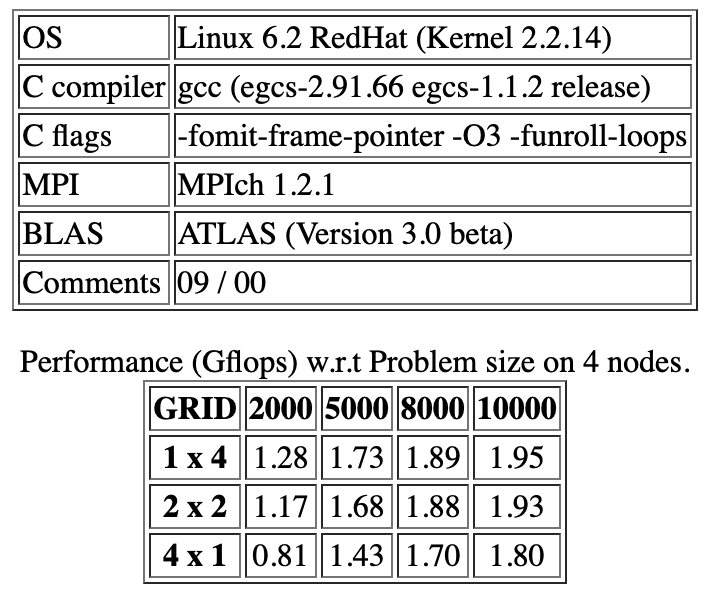
\includegraphics[width=0.95\linewidth]{ejemplo_HPL.png}
  \caption{Ejemplo oficial de tabla/salida de HPL (fuente: recurso oficial de HPL).}
  \label{fig:ejemplo_hpl}
\end{figure}

En esta tabla, los apartados más habituales significan:
\begin{itemize}
  \item \textbf{Columnas ($N$)}: los valores (p.ej. 2000, 5000, 8000, 10000, 15000, 20000) representan el \textbf{tamaño del problema} $N$, es decir, la dimensión de la matriz cuadrada $A$ del sistema denso aleatorio en doble precisión ($A\,x=b$). Al aumentar $N$, el rendimiento suele crecer hasta estabilizarse por un mejor aprovechamiento del cómputo.
  \item \textbf{Filas (GRID $P\times Q$)}: la primera columna \textit{GRID} indica la \textbf{rejilla de procesos} MPI $P\times Q$ (con $P$ filas y $Q$ columnas), de modo que el total de procesos es $P\cdot Q$; por ejemplo, $2\times 4=8$ procesos y $4\times 4=16$ procesos.
  \item \textbf{Celdas (GFLOPS)}: cada número de la tabla es el \textbf{rendimiento en GFLOPS} obtenido para esa combinación de tamaño $N$ y rejilla $P\times Q$.
\end{itemize}

\nocite{*}
\printbibliography[title={Bibliografía}]

\end{document}